\chapter{Contorno do problema e o ambiente de simulação}
\label{cha:problem-limits}

\section{Introdução}

Como Sperati et al. [\cite{sperati2011path}], abordamos o problema de formação de caminho utilizando robótica evolutiva. Cada robô é controlado por uma \textit{Time-Delay Neural Network} (Seção \ref{sec:tdnn}) e seus parâmetros são ajustados por algoritmos evolutivos (Seção \ref{sec:evolutionary-computation}).

A Seção \ref{sec:robots} descreve o robô utilizado para os estudos. A Seção \ref{sec:environment} descreve o ambiente a que esses robôs são submetidos. A Seção \ref{sec:fitness} define a função de \fitness que avalia a qualidade de uma solução para a instância do problema em questão. Por fim, a Seção \ref{sec:simulation} apresenta o ambiente de simulação desenvolvido e a motivação para tal feito.

\section{Os robôs}
\label{sec:robots}

O robô utilizado como referência é o \textit{e-puck} \cite{mondada2009epuck}, um pequeno robô cilíndrico com 7 centímetros de diâmetro. Dois motores independentes controlam duas rodas provendo tração diferencial e velocidade de até 8.2 cm/s. Oito sensores de luz infravermelha ao redor do robô permitem a detecção de obstáculos próximos (até aproximadamente 2.5 cm). Mais um sensor de luz infravermelha é colocado em baixo do robô para detecção da cor do chão (usado para diferenciar as áreas alvo do resto do ambiente). Além disso, o robô possuí uma câmera com alcance de 35 cm e campo de visão de $144\,^{\circ}$. Dois LEDs de cores diferentes na dianteira e traseira do robô, podendo ser acessos ou apagados, são detectáveis pela câmera de outros robôs permitindo uma forma de comunicação.

Para representar a informação captada pela câmera a codificamos em quatro valores binários: presença ou não de pontos azuis ou vermelhos (correspondendo aos LEDs dianteiros e traseiros, respectivamente) na região direita ou esquerda do campo de visão.

A estrutura da rede neural pode ser vista na Figura \ref{fig:robot-ann}. O conjunto de entradas da rede é composto por todos os sensores normalizados e o conjunto de saídas controla os dois motores e os dois LEDs. Vale observar que a configuração da rede (estrutura e pesos) é homogênea à todos os robôs do enxame.

\begin{figure}[H]
    \centering
    \includegraphics[width=0.8\textwidth]{figures/robot-ann}
    \caption{Rede neural controladora do robô}
    \label{fig:robot-ann}
\end{figure}

Matematicamente, a ativação $O_{j}$ do neurônio de saída $j$ no momento $t$ é computado pelas seguintes equações:

$$
O_{j}(t) = \sigma (\sum_{i} w_{ij}^{OI} I_{i}(t) + \sum_{i} w_{ij}^{OH} H_{i}(t) + \beta_{j}^{O})
$$
$$
H_{j}(t) = \tau_{j} \sigma (\sum_{i} w_{ij}^{HI} I_{i}(t) + \beta_{j}^{H}) + (1 - \tau_{j}) H_{j} (t - 1)
$$

onde $I_{i}$ é o valor da entrada $i$ (sensor normalizado). $\beta_{j}^{H}$ e $\beta_{j}^{O}$  representam o \textit{bias} relativo ao neurônio $j$ da camada intermediária e de saída, respectivamente. Finalmente, $w_{ij}^{OI}$, $w_{ij}^{OH}$ e $w_{ij}^{HI}$ são os pesos relativos a entrada $i$ e saída $j$ das sinapses que ligam, respectivamente, os neurônios: de entrada para saída, de entrada para intermediários e intermediários para saída.

O parâmetro denominado \textit{time constraint} ($\tau_{j}$) determina a fração de ativação do neurônios da camada escondida no momento anterior $H_{j} (t - 1)$ que é mantida no momento atual $H_{j} (t)$. Isso classifica a rede como uma \textit{Time-Delay Neural Network} visto que o histórico de ativação das entradas têm alguma influência na saída.

\section{O ambiente}
\label{sec:environment}

Os robôs são colocados em um espaço quadrado (250 cm de lado) delimitado por paredes. Dentro desse espaço, duas circunferências (16 cm de raio), denotadas por uma coloração escura (em contraste ao restante do espaço que apresenta coloração mais clara), representam as áreas alvo. O sensor de luz infravermelha localizado em baixo do robô é sensível à diferença de coloração, podendo assim perceber se está sobre uma área alvo ou não. Adicionalmente, no centro das áreas alvo, dois LEDs vermelhos sempre acessos são visíveis, indistinguivelmente, como os LEDs na traseira dos robôs.

\section{A função de \fitness}
\label{sec:fitness}

Seguindo o mesmo conceito apresentado por Sperati et al. \cite{sperati2011path}, a \fitness $F$ de uma solução $S$ é computada a partir de um teste com os robôs no ambiente físico por um determinado intervalo de tempo $T$. Dividimos esse intervalo em duas partes $T_{a}$ e $T_{b}$. Durante a primeira parte, a \fitness não é avaliada. A avaliação só começa a acontecer durante a segunda parte do teste.

No início do teste, cada robô $i$ ganha um valor virtual de energia $e_{i} = 2$. A função $\delta$ aproxima o consumo de energia a fim de que um robô, a máxima velocidade, consuma exatamente uma unidade de energia para mover-se de uma área alvo à outra.

$$
\delta_{i} (t) = \frac{( | \omega_{ir} (t) | + | \omega_{il} (t) |) r}{d}
$$

onde $r$ é o raio das rodas do robô, $d$ é a distância entre as áreas alvo e $\omega_{ir} (t)$ e $\omega_{il} (t)$ equivalem, respectivamente, à velocidade angular das rodas direita e esquerda do robô $i$ no momento $t$.

Na sequência, os seguintes passos são executados:

\begin{enumerate}
    \item A solução $S$ é aplicada ao enxame de robôs.
    \item Prepara-se o ambiente de testes, ou seja, as áreas alvo e os robôs são colocados em posições aleatórias dentro do ambiente.
    \item Os robôs são ligados e estão livres para mover-se dentro do ambiente sem afetar a \fitness durante a primeira parte do teste ($T_{a}$).
    \item Em seguida, inicia-se a segunda parte do teste ($T_{b}$) em que os robôs passam a ser avaliados da seguinte maneira:
    \begin{enumerate}
        \item A cada instante $t$, a energia de cada é robô é decrementada de $\delta (t)$.
        \item Se um robô entrar em uma área alvo, a energia restante é acrescida na \fitness individual e a energia volta a ser definida em 2.
    \end{enumerate}
    \item A \fitness individual é normalizada em relação ao máximo de viagens entre uma área alvo e outra que um robô poderia desempenhar (solução ótima).
    \item Finalmente, a \fitness do enxame é computada pela média de \fitness dos indivíduos que a compõe.
\end{enumerate}

Matematicamente,

$$
e_{i} (t) = \left\{
\begin{array}{l l}
1 & \quad \text{se o robô $i$ entrar em uma nova área alvo}\\
e_{i}(t - 1) - \delta_{i} (t) & \quad \text{caso contrário}
\end{array} \right.
$$

$$
f_{i} (t) = f_{i} (t - 1) + \left\{
\begin{array}{l l}
e_{i}(t - 1) & \quad \text{se o robô $i$ entrar em uma nova área alvo}\\
0 & \quad \text{caso contrário}
\end{array} \right.
$$

\noindent\begin{minipage}{.5\linewidth}
$$
F = \frac{1}{N} \sum_{i=1}^{N} f_{i} (T_{b}) / f_{max}
$$
\end{minipage}%
\begin{minipage}{.5\linewidth}
$$
f_{max} = \frac{2 \omega_{M} r T_{b}}{d}
$$
\end{minipage}\\

Assim, um robô que se move de uma área alvo a outra da maneira mais eficiente -- pelo menor caminho e a máxima velocidade -- mantêm exatamente uma unidade de energia toda vez que entrar em uma área alvo. Por consequência, sua \fitness individual será máxima (um) e, se todos os indivíduos apresentarem o mesmo comportamento, a \fitness do enxame também será máxima.

\section{O ambiente de simulação}
\label{sec:simulation}

Os algoritmos evolutivos utilizados na fase de treinamento necessitam de múltiplas avaliações da função de \fitness (na ordem das dezenas de milhar). Por esse motivo, a utilização de robôs reais em um ambiente físico é, apesar de possível, impraticável visto o tempo demandado por tal método. Além disso, não temos a disposição o número necessário de robôs para a realização dos experimentos. Assim, surge naturalmente a necessidade de um ambiente de simulação virtual que imite com fidelidade os robôs e o ambiente à que estes serão submetidos. Após o treinamento no ambiente simulado, a solução resultante -- parâmetros da rede neural -- poderá ser aplicada a um conjunto de robôs e esses demonstrarão o comportamento esperado.

O modelo mais comum de simulação baseia-se na aplicação de mecânica Newtoniana, porém Miglino et al. \cite{miglino1996evolving} aponta algumas dificuldades que podem ser encontradas com este tipo de simulador na fase de treinamento:
\begin{enumerate}
    \item Vários simuladores não consideram todas as leis da física envolvidas na interação entre agentes reais com o ambiente, por exemplo massa, peso, fricção, inércia etc.
    \item Sensores físicos retornam valores incertos e comandos enviados aos atuadores têm efeitos incertos. Em contraste, os ambientes de simulação geralmente retornam informações perfeitas.
    \item Diferentes sensores e atuadores, mesmo que aparentemente idênticos, podem apresentar pequenas mudanças mecânicas ou elétricas levando a diferentes comportamentos. Este fato é geralmente ignorado em simuladores.
\end{enumerate}

Estas dificuldades podem impedir a transição entre o ambiente de treinamento e o ambiente real.

Em seguida, Miglino et al. \cite{miglino1996evolving} propõe um modelo de simulação baseado em amostragem. Utilizando um robô no ambiente real, constrói-se uma tabela contendo amostragens do deslocamento linear e angular para diferentes valores aplicados aos atuadores. A partir daí, no simulador, as fórmulas de física clássica são substituídas por simples consultas nesta tabela. De forma análoga, os sensores do robô são amostrados para cada uma das diferentes classes de obstáculos presentes no ambiente.

Além disso, para aproveitar os recursos computacionais disponíveis, a simulação para o cálculo da função de \fitness é executada para todos os indivíduos da população de forma paralela pelo uso da plataforma \textit{OpenCL} \cite{amd2012amdaccelerated}. Essa plataforma fornece uma abstração de processamento e arquitetura de memória para desenvolvimento de programas que executam em diversos dispositivos como: \textit{central processing units} (CPUs), \textit{graphics processing units} (GPUs), \textit{digital signal processors} (DSPs) etc.

O modelo de programação \textit{Data-Parallel} é o foco primário da plataforma e tem como principal finalidade o desenvolvimento de programas para execução em GPGPUs\footnote{\textit{General Purpouse Graphics Processing Units} -- Unidades de processamento gráfico de propósito geral.}. Diferentemente do modelo padrão de programação em CPUs onde um instrução opera sobre um único item de dados (\textit{work-item}), no modelo \textit{Data-Parallel} cada instrução é executada paralelamente para um conjunto de dados (\textit{work-group}).

Assim, cada robô simulado corresponde a um \textit{work-item} e o conjunto de robôs pertences a um ambiente a um \textit{work-group}. A simulação e o cálculo da função de \fitness ocorre em paralelo para todos os robôs.